\documentclass[12pt]{article}

% Essential packages
\usepackage[utf8]{inputenc}
\usepackage[T1]{fontenc}
\usepackage{cancel}
\usepackage{amsmath}
\usepackage{mathtools}
\usepackage{graphicx}
\usepackage[margin=1in]{geometry}
\usepackage{algorithmic}
\usepackage{algorithm}
\usepackage{svg}
\usepackage{amssymb}

% Document information
\title{Tarea 2 - Análisis de algoritmos}
\author{David Rivera Morales \\ 320176876 \and José Antonio Gallegos Cortes \\ 320316566}
\date{\today}

\begin{document}

% Cover page
\begin{titlepage}
\begin{center}

% UNAM Logo
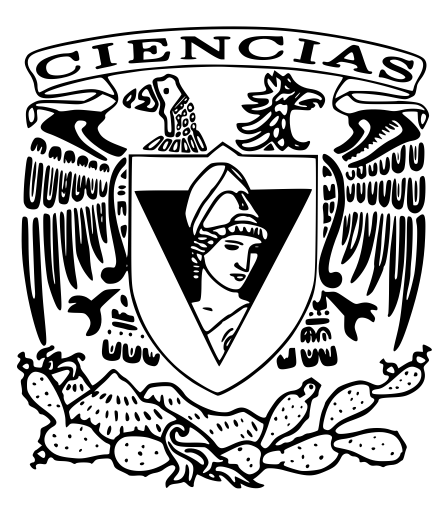
\includegraphics[width=0.3\textwidth]{images/escudo-unam.png}

\vspace{1cm}
{\Large UNIVERSIDAD NACIONAL AUTÓNOMA DE MÉXICO}

\vspace{1.5cm}
{\Large FACULTAD DE CIENCIAS}

\vspace{3cm}
{\Large Tarea 2}\\
\vspace{0.5cm}
{\Large Análisis de algoritmos}

\vspace{2cm}
\vspace{0.5cm}
{\large Rivera Morales David}\\
{\large 320176876}\\
\vspace{0.5cm}
{\large Gallegos Cortes José Antonio}\\
{\large 320316566}

\vfill
{\large \today}
\end{center}
\end{titlepage}

\section*{Solución de los 8 pares de funciones}

% Nota: Recordamos que para el análisis asintótico se considera el comportamiento cuando \( n \to \infty \).

\begin{enumerate}

  \item \textbf{Par 1:} 
  % Definición de las funciones f(n) y g(n).
  \[
    f(n) = \log(n), \quad g(n) = \log\bigl(n^2 + 1\bigr).
  \]
  % Explicación paso a paso:
  % 1. Se observa que para n grande, el término 1 en n^2 + 1 es insignificante respecto a n^2.
  % 2. Por ello, se tiene que \( n^2 + 1 \sim n^2 \) cuando \( n \to \infty \).
  % 3. Usando la propiedad de los logaritmos: \(\log(n^2) = 2\log(n)\).
  % 4. Así, ambos términos se comportan como \(2\log(n)\) para n suficientemente grande.
  % 5. Al formar el cociente, se obtiene una constante positiva, lo que implica que f(n) y g(n) tienen el mismo orden de crecimiento.
  \textbf{Análisis:} \\
  Vamos a resolver el limite $\lim_{n \to \infty} \frac{f(n)}{g(n)}$ y dependiendo del resultado podremos determinar que complejidad tiene, si tenemos que el limite es igual a 0 entonces f(n)$\in$o(g(n)), si es mayor a cero pero menor a infinito tendremos que f(n)$\in \theta$(g(n)) y por último si tenemos que es infinito entonces f(n)$\in \omega$(g(n))
  por lo que tenemos lo siguiente: \\
  $\lim_{n \to \infty} \frac{log(n)}{log(n^2+1)} = \lim_{n \to \infty} \frac{\frac{1}{n}}{\frac{2n}{n^2+1}}$ por L'hopital. \\ Y seguimso desarrollando la expresión:
  \[\lim_{n \to \infty} \frac{\frac{1}{n}}{\frac{2n}{n^2+1}} = \lim_{n \to \infty} \frac{n^2+1}{2n^2} \text{ podemos sacar la constante } \frac{1}{2}, \text{ tenemos entonces: } \frac{1}{2}\lim_{n \to \infty} \frac{n^2+1}{n^2}
  \]
  Ahora podemos separar la división: 
  \[\frac{1}{2}\lim_{n \to \infty} \frac{n^2}{n^2}+\frac{1}{n^2} = \frac{1}{2}\lim_{n \to \infty} \frac{\cancel{n^2}}{\cancel{n^2}}+\frac{1}{n^2} = \frac{1}{2}\lim_{n \to \infty} 1+ \frac{1}{n^2}
  \]
  Finalmente podemos separar en dos limites:
  \[
  \frac{1}{2}(\lim_{n \to \infty} 1 +\lim_{n \to \infty} \frac{1}{n^2})
  \]
  El limite de una constante es la constante, mientras que para el limite de $\frac{1}{n^2}$ si aplicamos la propiedad $\lim {n \to \infty} (\frac{c}{n^a}) =0$ por lo que al final tenemos:
  \[
  \frac{1}{2}(1+0) = \frac{1}{2}
  \]
  Como es mayor que cero y menor que infinito sabemos que $f(n)\in \theta (g(n))$

  \item \textbf{Par 2:} 
  % Definición de las funciones.
  \[
    f(n) = \frac{n^2}{\log(n)}, \quad g(n) = n(\log(n))^2.
  \]
  % Explicación:
  % 1. Aplicamos la propiedad logarítmica: \(\log(n^2)= 2\log(n)\).
  % 2. Así, g(n) es simplemente 2 veces f(n), es decir, un múltiplo constante de f(n).
  % 3. Al calcular el cociente, se obtiene \(\frac{1}{2}\), lo que es una constante positiva.
  \textbf{Análisis:}\\
  Por $\frac{\frac{b}{c}}{a} = \frac{b}{c*a}$
  \[
  \lim_{n \to \infty} \frac{\frac{n^2}{\log(n)}}{n(\log(n))^2} =  \lim_{n \to \infty} \frac{n^2}{\log(n)(n\log(n))^2} \text{ por } (ab)^c = a^cb^c \text{ tenmos que} \lim_{n \to \infty} \frac{n^2}{n^2\log^2(n)\log(n)}
  \]
  Ahora sumamos los exponentes y dividimos las $x^2$
  \[
   \lim_{n \to \infty} \frac{\cancel{n^2}}{\cancel{n^2}\log^3(n)} = \lim_{n \to \infty} \frac{1}{\log^3(n)} = \frac{\lim_{n \to \infty} 1}{\lim_{n \to \infty} \log^3(n)} = \frac{1}{\infty ^3} = \frac{1}{\infty} = 0
  \]
  
  Por ello:
  \[
    f(n)\in o(g(n))
  \]

  \item \textbf{Par 3:} 
  % Definición de las funciones.
  \[
    f(n) = (n^3)2^n, \quad g(n) = n3^n.
  \]
  % Explicación:
  % 1. Se observa que \(n^6\) es \(n^3\) elevado al cuadrado, por lo que crece mucho más rápido que \(n^3\).
  % 2. Al formar el cociente se tiene:
  \[
    \frac{f(n)}{g(n)} = \frac{(n^3)2^n}{n3^n}.
  \]
  % 3. Como \(n^3 \to \infty\) cuando \(n \to \infty\), se concluye que f(n) crece asintóticamente mucho más rápido que g(n).
  \textbf{Análisis:}
  \[
  \lim_{n \to \infty} \frac{(n^\cancel{3})2^n}{\cancel{n}3^n} = \lim_{n \to \infty} \frac{(n^2)2^n}{3^n} = \lim_{n \to \infty} (n^2)\frac{2^n}{3^n} = \lim_{n \to \infty} (n^2)(\frac{2}{3})^n
  \]
  Reescribimos con la propiedad $a*b = \frac{a}{\frac{1}{b}}$ para usar L'hopital, la raíz de $n^2$ es $2n$ mientras que la de $\frac{1}{(\frac{2}{3})^n}$ la obtendremos ahora
  \[
  (\frac{1}{(\frac{2}{3})^n})'= ((\frac{3}{2})^n)´= (\frac{3}{2})^nlog(\frac{3}{2})
  \]
  Por lo que debemos obtener el limite de $\lim_{n \to \infty} \frac{2n}{(\frac{3}{2})^nlog(\frac{3}{2})}$, aplicamos L'hopital y sacamos las derivadas
  \[
  \lim_{n \to \infty} \frac{(2n)´}{(\frac{3}{2})^nlog(\frac{3}{2})´} = \frac{2}{log(\frac{3}{2})\frac{d}{dx}(\frac{3}{2})^n)} = \frac{2}{log(\frac{3}{2})(\frac{3}{2})^nlog(\frac{3}{2})} = \frac{2}{log^2(\frac{3}{2})(\frac{3}{2})^n}
  \]
  Ahora simplificamos con la misma propiedad $a*b = \frac{a}{\frac{1}{b}}$ y usamos la propiedad $\frac{a}{\frac{b}{c}} = \frac{a*c}{b}$ para luego poder sacar casi toda la expresión como una constante.
  \[
  \lim_{n \to \infty} \frac{2}{log^2(\frac{3}{2})(\frac{3^n}{2^n})} = \frac{2}{\frac{log^2(\frac{3}{2})(3^n)}{2^n}} = \frac{2*2^n}{log^2(\frac{3}{2})3^n} = \frac{2}{log^2(\frac{3}{2})} * \frac{2^n}{3^n}
  \]
  Sacamos como una constante y aplicamos la regla $\frac{a^c}{b^c}=\frac{a}{b}^c$
  \[
  \frac{2}{log^2(\frac{3}{2})} \lim_{n \to \infty} (\frac{2^n}{3^n}) = \frac{2}{log^2(\frac{3}{2})} \lim_{n \to \infty} (\frac{2}{3})^n = \frac{2}{log^2(\frac{3}{2})}*0 = 0
  \]
  Como es cero tenemos que $f(n)\in o(g(n))$    

  \item \textbf{Par 4:} 
  % Definición de las funciones.
  \[
    f(n) = n!, \quad g(n) = n^{n}.
  \]
  % Explicación:
  % 1. Se aplica la propiedad logarítmica: \(\log(n^2)= 2\log(n)\), obteniéndose:
  \[
    f(n) = n \cdot 2\log(n)= 2n\log(n).
  \]
  % 2. Como g(n) = n log(n), el cociente es:
  \[
    \frac{f(n)}{g(n)} = \frac{2n\log(n)}{n\log(n)} = 2.
  \]
  % 3. El cociente constante implica que ambas funciones tienen el mismo orden de crecimiento.
  \textbf{Análisis:}
  \[
    f(n) \in \Theta\bigl(g(n)\bigr).
  \]

  \item \textbf{Par 5:}
  % Definición de las funciones.
  \[
    f(n) = \log\bigl(\log(n)\bigr), \quad g(n) = \sqrt{\log(n)}.
  \]
  % Explicación:
  % 1. La función \(\log(n)\) tiende a infinito al crecer \(n\), pero de manera lenta.
  % 2. La función \(f(n)\) toma el logaritmo de \(\log(n)\), lo que ralentiza aún más su crecimiento.
  % 3. En cambio, \(g(n)=\sqrt{\log(n)}\) equivale a \((\log(n))^{1/2}\), que crece más rápido que \(\log(\log(n))\).
  % 4. Para ver esto, se forma el cociente:
  \[
    \frac{f(n)}{g(n)} = \frac{\log(\log(n))}{(\log(n))^{1/2}}.
  \]
  % 5. Al tomar el límite cuando \(n \to \infty\), el denominador domina al numerador, y el límite es 0.
  \textbf{Análisis:}
  Vamos a hacer un cambio de variable, vamos a cambiar $\log n$ por t para luego aplicar L´hopital, por lo que nos quedaría como:
  \[
  \lim_{x \to \infty} \frac{\log(t)}{t^{\frac{1}{2}}} = \frac{\log(t)´}{t^{\frac{1}{2}´}} = \frac{\frac{1}{t}}{\frac{1}{2}t^{-1/2}} = \frac{\frac{1}{t}}{\frac{1}{2t^{1/2}}} = \frac{2t^{1/2}}{t} 
  \]
  Aplicamos las leyes de los exponentes $\frac{x^a}{x^b}= \frac{1}{x^{b-a}}$
  \[
  \lim_{x \to \infty} \frac{2}{t^{1-1/2}} = \lim_{x \to \infty} \frac{2}{t^{1/2}} \text{ aplicamos la propiedad } lim_{x \to \infty}(\frac{c}{x^a})= 0
  \]
  y como tenemos que el limite es cero entonces:    
  % Concluimos que f(n) crece mucho más despacio que g(n).
  \[
    f(n) \in o\bigl(g(n)\bigr).
  \]

  \item \textbf{Par 6:}
  % Definición de las funciones.
  \[
    f(n) = n^{\log(n)}, \quad g(n) = n \,\log(n) - n.
  \]
  % Explicación:
  % 1. Se simplifica g(n) factorizando n: 
  \[
    g(n) = n\bigl(\log(n)-1\bigr).
  \]
  % 2. Para n grande, \(\log(n)-1\) es positivo, por lo que g(n) se comporta como \(n\log(n)\).
  % 3. Para f(n), se utiliza la transformación exponencial:
  \[
    n^{\log(n)} = \exp\bigl(\log(n)\cdot\log(n)\bigr)= \exp\bigl((\log(n))^2\bigr).
  \]
  % 4. Se compara el crecimiento de \(\exp\bigl((\log(n))^2\bigr)\) con \(n\log(n)\) formando el cociente:
  \[
    \frac{f(n)}{g(n)} \approx \frac{\exp\bigl((\log(n))^2\bigr)}{n\,\log(n)}.
  \]
  % 5. Tomando logaritmos del cociente para simplificar la comparación:
  \[
    \log\!\Bigl(\frac{f(n)}{g(n)}\Bigr) \approx (\log(n))^2 - \log\bigl(n\,\log(n)\bigr).
  \]
  % 6. Se nota que \((\log(n))^2\) domina a \(\log(n) + \log(\log(n))\) (recordando que \(\log\bigl(n\,\log(n)\bigr) = \log(n) + \log(\log(n))\)).
  % 7. Esto implica que el cociente tiende a infinito, demostrando que f(n) crece mucho más rápido que g(n).
  \textbf{Análisis:}
  \[
    \lim_{n\to\infty} \frac{f(n)}{g(n)} = \infty.
  \]
  Por lo tanto,
  \[
    f(n) \in \omega\bigl(g(n)\bigr).
  \]

  \item \textbf{Par 7:}
  % Definición de las funciones.
  \[
    f(n) = log(n\sqrt{n}), \quad g(n) = \sqrt{n} \log(n)
  \]
  % Explicación:
  % 1. Aplicamos la propiedad logarítmica para f(n): 
  % 4. Dado que tanto \(n^{1/2}\) como \((\log(n))^{3/2}\) tienden a infinito al crecer n, su producto también lo hace.
  \textbf{Análisis:}
  Aplicando las leyes de los exponentes $\frac{1}{a^b}=a^-b$
  \[
  \lim_{n \to \infty}(\frac{ln(n\sqrt{n})}{\sqrt{n}ln(n)}) = \lim_{n \to \infty}(\frac{ln(nn^{1/2})}{\sqrt{n}ln(n)}) = \lim_{n \to \infty}(\frac{ln(n^{3/2})}{\sqrt{n}ln(n)})= \lim_{n \to \infty}(\frac{\frac{3}{2}ln(n)}{\sqrt{n}ln(n)}) = 
  \]
  \[
  \lim_{n \to \infty}(\frac{3\cancel{ln(n)}}{2\sqrt{n}\cancel{ln(n)}}) = \lim_{n \to \infty}(\frac{3}{2\sqrt{n})}) = \frac{3}{2} \frac{\lim_{n \to \infty} 1}{\lim_{n \to \infty}\sqrt{n}} = \frac{3}{2}\frac{1}{\sqrt{\infty}} =\frac{3}{2} \frac{1}{\infty} = \frac{3}{2}*\frac{1}{\infty} = \frac{3}{2}*0 = 0
  \]
  
  Así,
  \[
    f(n) \in o\bigl(g(n)\bigr).
  \]

  \item \textbf{Par 8:}
  % Definición de las funciones.
  \[
    f(n) = 2^{\,n^2 + 1}, \quad g(n) = 4^n.
  \]
  \textbf{Análisis:}
  % Explicación:
  % 1. Se reescribe \(g(n)\) en base 2 utilizando que \(4 = 2^2\):
  \[
    4^n = (2^2)^n = 2^{2n}.
  \]
  % 2. Así, f(n) se expresa como \(2^{\,n^2+1}\) y g(n) como \(2^{2n}\).
  % 3. Se comparan los exponentes: \(n^2 + 1\) crece mucho más rápido que \(2n\) para n grande.
  % 4. Al formar el cociente:
  \[
    \frac{f(n)}{g(n)} = \frac{2^{n^2+1}}{2^{2n}} = 2^{\,n^2 + 1 - 2n}.
  \]
  % 5. Se simplifica el exponente:
  \[
    n^2 + 1 - 2n = n^2 - 2n + 1
  \]
  Por lo que ahora simplemente calculamos el limite de lo anterior con la propiedad de los limites que nos dice que dado un polinomio \( P(x) = (a_n x^n  + \dots + bx+c) \), el límite  \(\lim_{x \to \infty} (a_n x^n  + \dots + bx+c) = \infty, a>0\) como en nuestro caso tenemos $a=1$ y $n=2$ 
  \[
  \lim_{n \to \infty} n^2 - 2n + 1 = \infty
  \]
  
  % 6. Como \((n-1)^2\) tiende a infinito, \(2^{(n-1)^2}\) también lo hace, lo que implica que f(n) crece asintóticamente más rápido.
  Como tenemos que es infinito entonces sabemos que:
  \[
    f(n) \in \omega\bigl(g(n)\bigr).
  \]

\end{enumerate}

\end{document}

